% \section{Praktiken}

In der Fachpraxis haben sich einige Technologien über die Jahre entwickelt und etabliert, welche die Nachvollziehbarkeit von Anwendungsverhalten und Nutzerinteraktion ermöglichen oder verbessern. Auf Basis der zuvor vorgestellten Methoden und teils neuer Ansätze haben sich in der Wirtschaft einige Praktiken entwickelt. Diese werden folgend näher beleuchtet.

\subsection{System Monitoring}

System Monitoring beschäftigt sich mit der Überwachung der notwendigen Systeme und Dienste in Bezug auf Hardware- und Softwareressourcen. Es handelt sich hierbei um ein projektunabhängiges Monitoring, welches sicherstellen soll, dass die Infrastruktur funktionstüchtig bleibt.

Ein Beispiel für System Monitoring wäre u. A., wenn man eine Menge an Systemen auf die Festplatten- und CPU-Auslastung hin kontrolliert und überwacht. Es können weitere Aspekte überwacht werden, aber im Regelfall hat die Überwachung selbst nichts mit einem eigentlichen Projekt zu tun, außer dass die Infrastruktur hierfür sichergestellt wird.

\subsection{Log Management}

Log Management umfasst die Erfassung, Speicherung, Verarbeitung und Analyse von Logdaten von Anwendungen. Neben diesen Funktionen bieten solche Werkzeuge oftmals fundierte Suchfunktionen und Visualisierungsmöglichkeiten. Um die Daten aus einer Anwendung heraus zu exportieren, gibt es meist eine Vielzahl an Integrationen für Frameworks und Logbibliotheken.

Einer der wichtigsten Punkte beim Log Management, ist der Umgang mit großen Datenmengen und die gewünschten Operationen, die Nutzer damit durchführen möchten.

\subsection{Application Performance Monitoring (APM)}

Beim Application Performance Monitoring werden Messdaten innerhalb von Anwendungen gesammelt, um das Anwendungsverhalten nachvollziehbar zu gestalten \cite{StudyingTheEffectivenessOfAPMTools}. Beispielsweise werden Aufrufe von Schnittstellen näher beleuchtet und die Antwortzeit gespeichert. Auf Basis der Daten lassen sich u. A. Abweichungen von der Norm feststellen, von einzelnen Systemen oder vom aktuellen Gesamtsystem zu einem vorherigen Zeitpunkt.

Mithilfe von APM lassen sich allgemeine Aspekte von Software, wie die Ressourcennutzung, überprüfen aber auch spezielle Faktoren, wie die Ausführungszeit einer wichtigen Methode, lassen sich so beleuchten. Die zu veranschaulichenden Aspekte werden zum Großteil über Metriken in numerische Werte abgebildet.

\subsection{Real User Monitoring (RUM)}

\nomenclature[Fachbegriff]{UI}{User-Interface}

Real User Monitoring beschäftigt sich mit dem Mitschneiden von allen Nutzerinteraktionen und Umgebungseigenschaften einer Benutzeroberfläche \cite{IdentifyingWebPerformanceDegradations}. Hiermit lässt sich nachvollziehen, wie ein Nutzer die Anwendung verwendet. RUM kann weiterhin dazu verwendet werden, um nachzuvollziehen, wie ein Zustand vom Nutzer erreicht worden ist. Aber es können auch ineffiziente Klickpfade hierdurch festgestellt werden und darauf basierend UX-Verbesserungen vorgenommen werden.

Weiterhin ist es beim RUM auch üblich Nutzerinteraktionen gruppierte zu analysieren, um verbreitete und unübliche Sitzungen zu identifizieren. Hiermit wird die Nutzerschaft und ihre Verhaltensweisen nachvollziehbarer gemacht.

%\subsection{Synthetic Monitoring}
%
%Beim Synthetic Monitoring werden Endnutzer simuliert, um Aspekte wie Funktionalität oder Verfügbarkeit zu verifizieren \cite{IdentifyingWebPerformanceDegradations}. Hierbei können Werkzeuge zur Browserautomatisierung eine echte Benutzung einer Webanwendung simulieren. Des Weiteren ist aber auch eine Nachstellung des Verhaltens der Webanwendung eine Option, indem z. B. Aufrufe zu Partnersystemen simuliert werden.

\subsection{Error Monitoring}

Das Error Monitoring konzentriert sich auf das Erfassen und Melden von Fehlern \cite{CrashbinCrashMonitoring}. Neben den eigentlichen Fehlern werden meist alle verfügbaren Kontextinformationen mit erfasst. Darunter finden sich u. A. Daten aus den Gebieten RUM und Logging. Das Error Monitoring wird oftmals eng mit einem Issue-Management verbunden, um aufgetretene Fehler und deren Behebung nachvollziehbar zu machen \cite{CrashbinCrashMonitoring}.

\subsection{Session-Replay}

Session-Replay beschreibt das Vorgehen, eine Sitzung eines Nutzers nachzustellen, so als ob sie gerade passiert \cite{NoBoundariesExfiltrationBySessionReplayScripts}. Hierbei können einzelne Aspekte der Anwendung nachgestellt werden, bspw. der Kommunikationsablauf oder die DOM-Manipulationen. Je mehr Aspekte nachgestellt werden, desto realitätsnaher ist die Nachstellung und entsprechend hilfreich ist sie beim Nachvollziehen.

Realitätsnahes Session-Replay nimmt somit eine enorme Datenmenge für jede Nutzersitzung auf und benötigt besonders bei Browsern eine effiziente Kommunikation, um die UX nicht negativ zu beeinflussen.

\begin{wrapfigure}[10]{r}{0.40\textwidth}
\centering
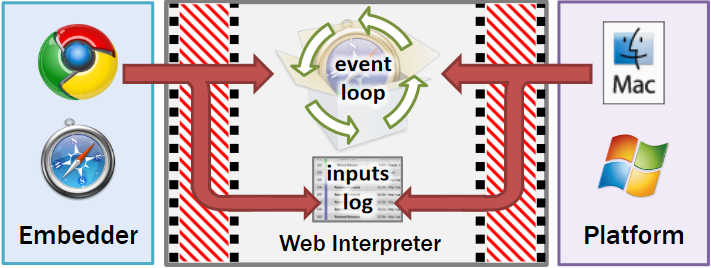
\includegraphics[width=\linewidth]{img/03_methoden/timelapse_figure5.png}
\caption{Mitschneiden von DOM-Events, Abb. aus \cite{TimelapsePaper}}
\label{fig:timelapse_figure5}
\end{wrapfigure}

Bereits 2013 entwickelten Burg \etal \cite{TimelapsePaper} mit \enquote{Timelapse} ein Framework, um Benutzersitzungen bei Webanwendungen aufzunehmen und wiederzugeben. Timelapse unterscheidet sich zu gängigen Session-Replay-Ansätzen dahingehend, dass die Wiedergabe keine vereinfachte Nachstellung der Anwendung ist. Stattdessen wird die JavaScript-Eventloop abgekapselt und es werden die Aufrufe von und zu der Eventloop mitgeschnitten (vgl. \autoref{fig:timelapse_figure5}).

\begin{wrapfigure}[10]{r}{0.40\textwidth}
\centering
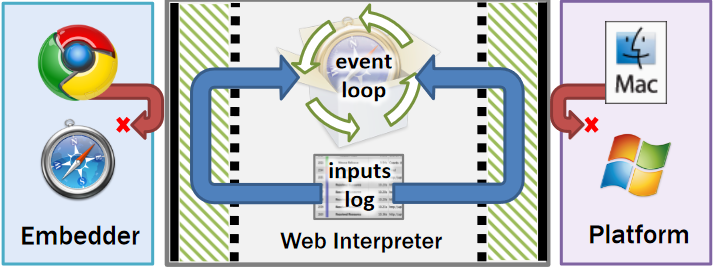
\includegraphics[width=\linewidth]{img/03_methoden/timelapse_figure6.png}
\caption{Abspielen von DOM-Events, Abb. aus \cite{TimelapsePaper}}
\label{fig:timelapse_figure6}
\end{wrapfigure}

Beim Abspielen werden die Aufrufe dann in derselben Reihenfolge an die Eventloop übergeben (vgl. \autoref{fig:timelapse_figure6}). Dies bedeutet es ist ein exaktes wiederholtes Ausführen in derselben Umgebung möglich und dies ermöglicht eine detaillierte Nachvollziehbarkeit des Anwendungsverhaltens. Leider wird für diesen Ansatz eine gepatchte Version von WebKit vorausgesetzt, somit wird auch Zugriff auf das Endnutzersystem benötigt. Aus diesem Grund und weil es sehr mehr als 5 Jahren nicht mehr gepflegt wird\footnote{Timelapse GitHub Repo \url{https://github.com/burg/replay-staging/}}, ist es ungeeignet für die hier angestrebte Lösung. Die vorgestellten Konzepte stellen jedoch nützliche Kernprinzipien für das Session Replay im Allgemeinen dar.

\subsection{OpenTelemetry}
\label{subsec:opentelemetry}

OpenTelemetry (OTel) \cite{OpenTelemetry} ist ein sich derzeit\footnote{Ein erster (General-Availability-)Release der Spezifikation ist für Q1 2021 geplant \cite{OpenTelemetryGARelease}.} entwickelnder herstellerunabhängiger Standard, um Tracing-, Metrik- und Logdaten\footnotemark{} zu erfassen, zu verarbeiten, zu analysieren und zu visualisieren. OTel fasst die beiden Standards OpenTracing und OpenCensus \cite{OpenCensus} zusammen und hat sich als Ziel gesetzt diese zu erweitern \cite{UseNixDistributiveTracing}. Hinter dem Standard stehen u. A. die Cloud Native Computing Foundation (CNCF), Google, Microsoft, und führende Hersteller von Tracing- und Monitoring-Lösungen.

Ziel ist es, dass Entwickler Tools und Werkzeuge benutzen können, ohne erneut hochspezifische Anbindungen schreiben und konfigurieren zu müssen. Stattdessen definiert der Standard Komponenten, die spezielle Aufgabengebiete haben und mit einer allgemeinen API anzusprechen sind. Die technische Infrastruktur einer auf OTel basierenden Lösung ist in \autoref{fig:otel-unified-collection} zu sehen. Im groben definiert OTel folgende Komponenten: API, SDK, Exporter, Collector und Backend (vgl. \autoref{fig:otel-components}).

\nomenclature[Fachbegriff]{OTel}{OpenTelemetry}
\nomenclature[Fachbegriff]{CNCF}{Cloud Native Computing Foundation}
\footnotetext{Eine Entwicklung einer Definition zu Logging ist im Gange \cite{OpenTelemetryLoggingSpecification}.}

\begin{figure}[H]
	\centering
	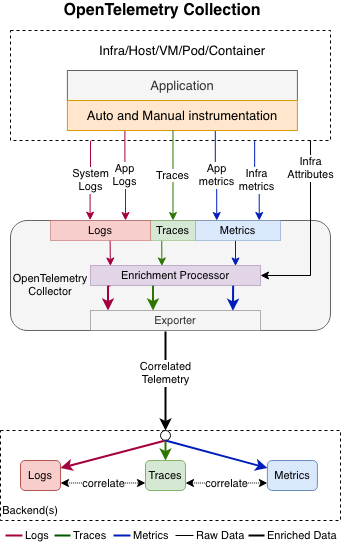
\includegraphics[width=\linewidth]{img/03_methoden/otel_unified-collection_2.png}
	\caption{Schaubild einer Lösung auf Basis von OTel \cite{OpenTelemetryUnifiedCollection}}
	\label{fig:otel-unified-collection}
\end{figure}

\begin{figure}[H]
	\centering
	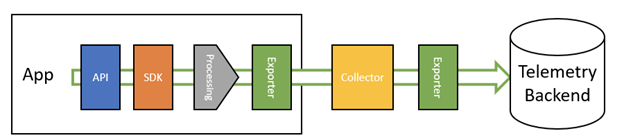
\includegraphics[width=0.75\linewidth]{img/03_methoden/dynatrace_otel-components.png}
	\caption{OTel Komponenten \cite{DynatraceOTelComponents}}
	\label{fig:otel-components}
\end{figure}